% !TEX TS-program = pdflatex
% !TEX encoding = UTF-8 Unicode

% This is a simple template for a LaTeX document using the "article" class.
% See "book", "report", "letter" for other types of document.

\documentclass[12pt]{article} % use larger type; default would be 10pt

\usepackage[utf8]{inputenc} % set input encoding (not needed with XeLaTeX)
\usepackage{amssymb}
%%% Examples of Article customizations
% These packages are optional, depending whether you want the features they provide.
% See the LaTeX Companion or other references for full information.

%%% PAGE DIMENSIONS
\usepackage{geometry} % to change the page dimensions
\usepackage{setspace}
\geometry{a4paper} % or letterpaper (US) or a5paper or....
\geometry{margin=1in} % for example, change the margins to 2 inches all round
% \geometry{landscape} % set up the page for landscape
%   read geometry.pdf for detailed page layout information

\usepackage{graphicx} % support the \includegraphics command and options

% \usepackage[parfill]{parskip} % Activate to begin paragraphs with an empty line rather than an indent

%%% PACKAGES
\usepackage{booktabs} % for much better looking tables
\usepackage{array} % for better arrays (eg matrices) in maths
\usepackage{paralist} % very flexible & customisable lists (eg. enumerate/itemize, etc.)
\usepackage{verbatim} % adds environment for commenting out blocks of text & for better verbatim
\usepackage{subfig} % make it possible to include more than one captioned figure/table in a single float
% These packages are all incorporated in the memoir class to one degree or another...

%%% HEADERS & FOOTERS
\usepackage{fancyhdr} % This should be set AFTER setting up the page geometry
\pagestyle{fancy} % options: empty , plain , fancy
\renewcommand{\headrulewidth}{0pt} % customise the layout...
\lhead{}\chead{}\rhead{}
\lfoot{}\cfoot{\thepage}\rfoot{}

%%% SECTION TITLE APPEARANCE
\usepackage{sectsty}
\allsectionsfont{\sffamily\mdseries\upshape} % (See the fntguide.pdf for font help)
% (This matches ConTeXt defaults)

%%% ToC (table of contents) APPEARANCE
\usepackage[nottoc,notlof,notlot]{tocbibind} % Put the bibliography in the ToC
\usepackage[titles,subfigure]{tocloft} % Alter the style of the Table of Contents
\renewcommand{\cftsecfont}{\rmfamily\mdseries\upshape}
\renewcommand{\cftsecpagefont}{\rmfamily\mdseries\upshape} % No bold!

%%% END Article customizations

%%% The "real" document content comes below...

\title{1.3 Bond Enthalpy}
\author{Peter Zhang}
%\date{} % Activate to display a given date or no date (if empty),
         % otherwise the current date is printed 

\doublespacing
\begin{document}
\maketitle

\pagebreak

\tableofcontents

\pagebreak

% start document
\section {Bond Enthalpy}

Bond enthalpy is is the energy required to break bonds

Bond Enthalpy's are actually `average` values, not exact values. This is why sometimes we opt to use Hess's Law over Bond Enthalpy Formulas due to inaccuracies in average values.

\begin{figure}[h]
	\centering
	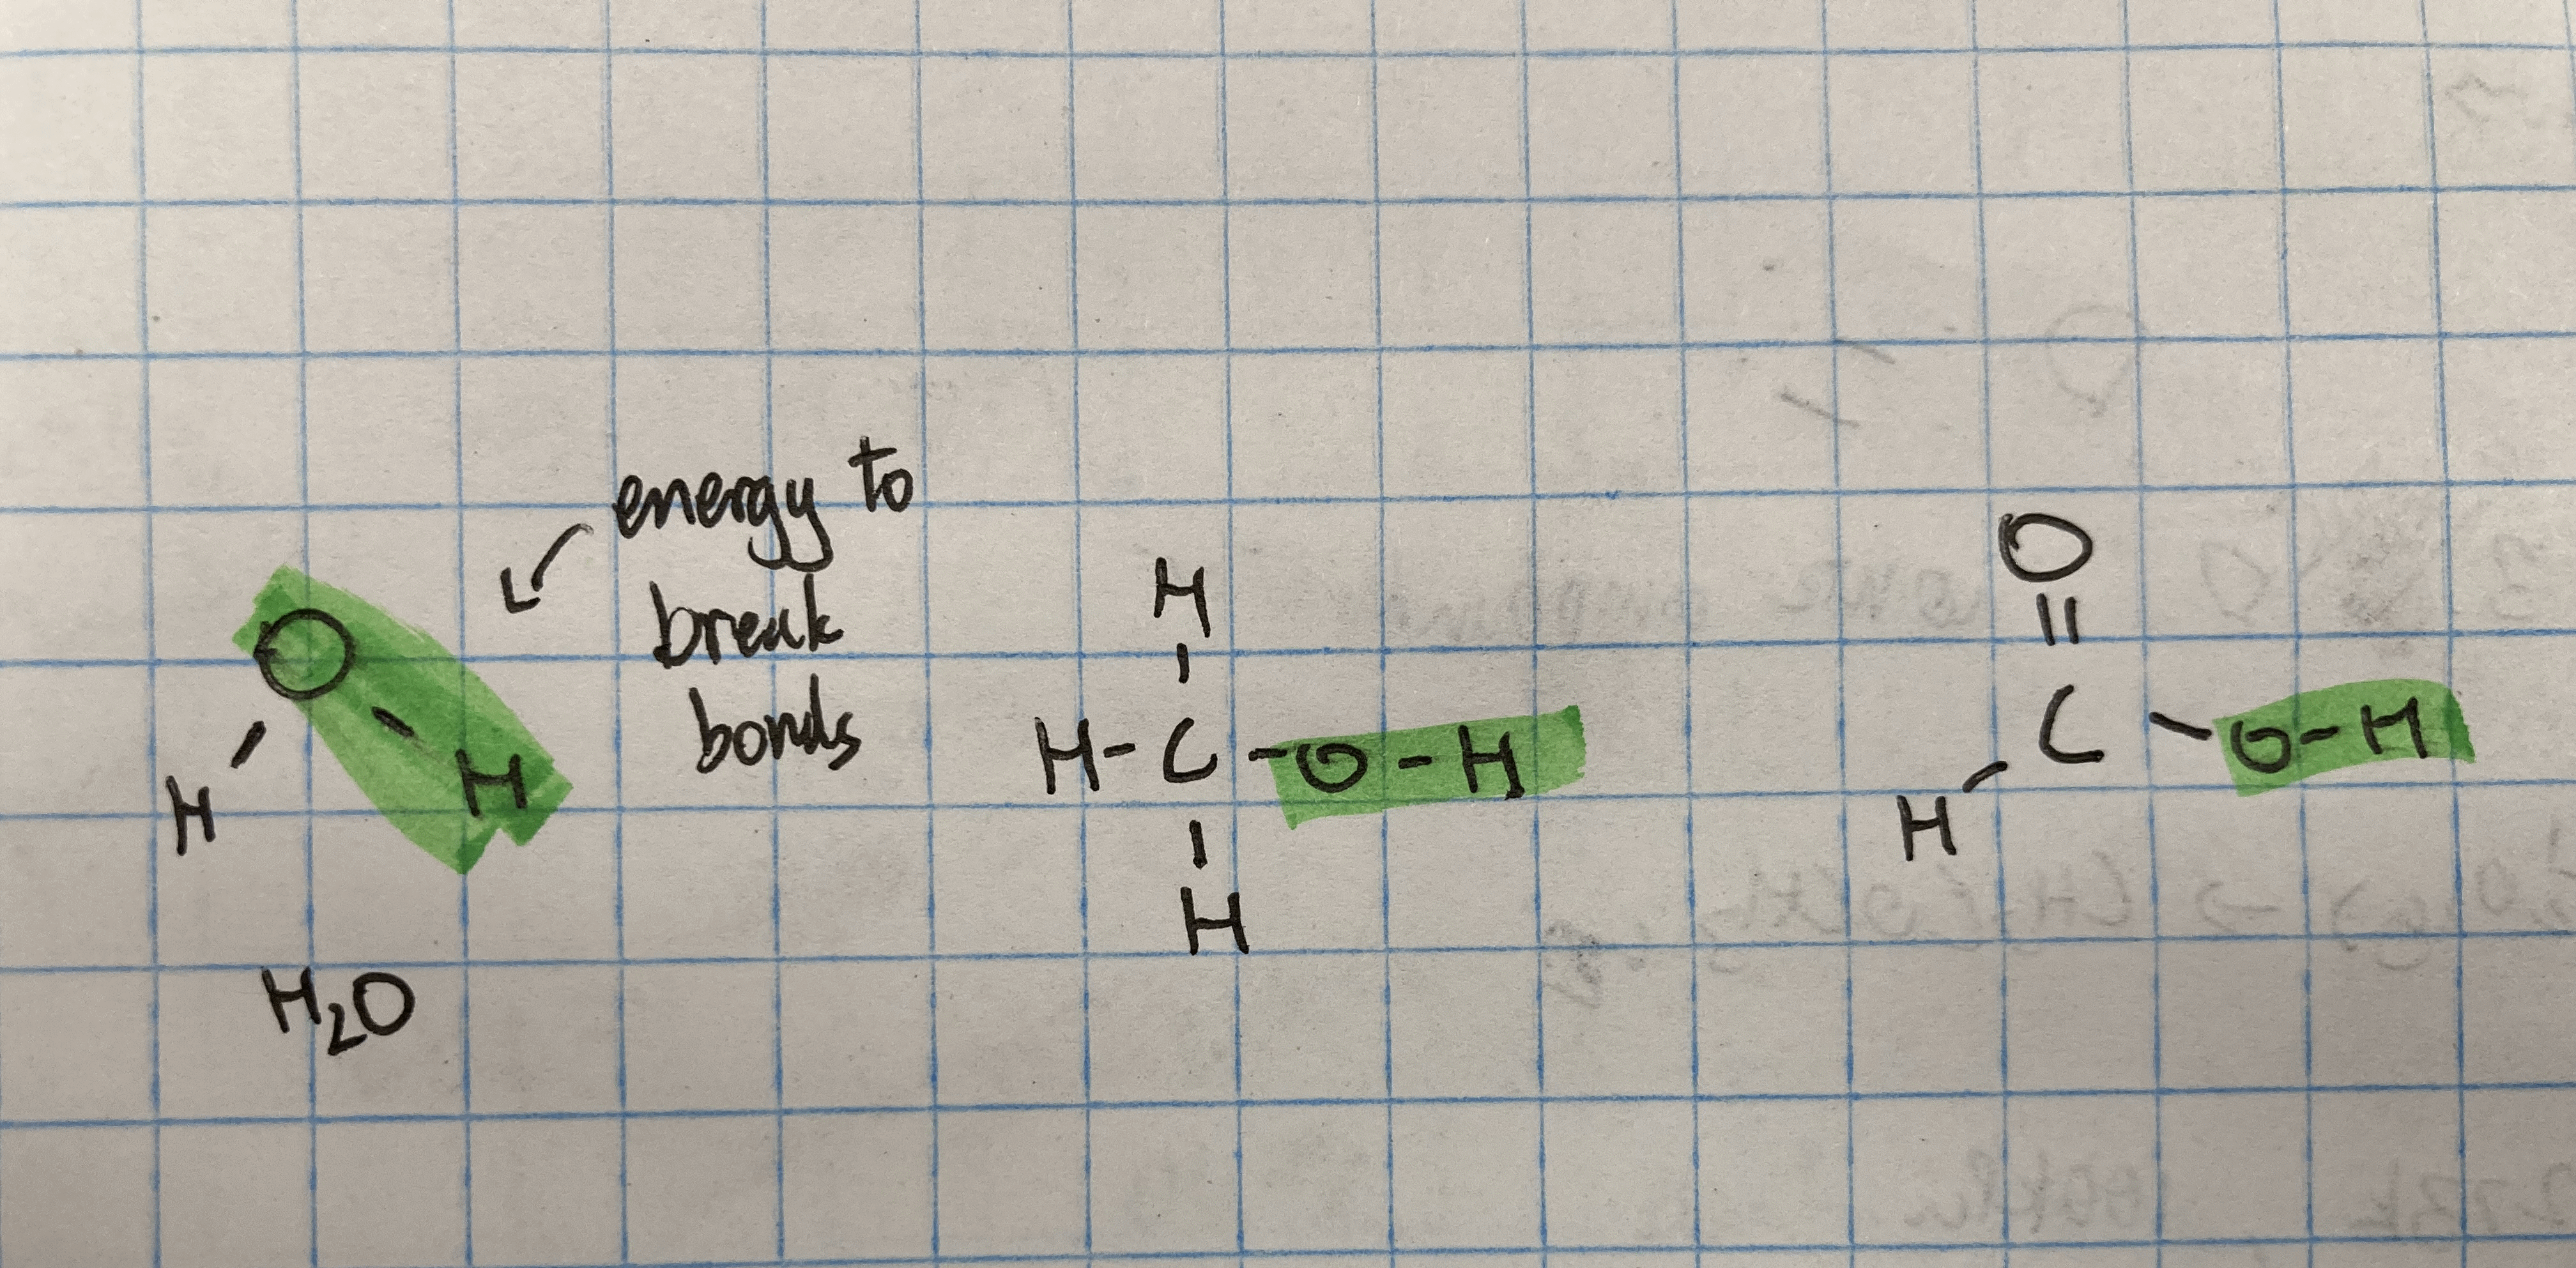
\includegraphics[width=\textwidth]{../images/1.3fig1.png}
	\caption{Bond Enthalpy in certain atoms}
	\label{fig:image}
\end{figure}

Enthalpy values from Bond Enthalpy equations will not equal the value from Hess's Law.

\subsection{Bond Enthalpy Equation}

\textbf{Equation (similar to Formation Enthalpy)}

$$\triangle{H} = \sum{\triangle{H}_{bonds\ broken(reactants)}} - \sum{\triangle{H}_{bonds\ formed(products)}}$$

\pagebreak

\subsection{Example}

How to solve the following?

\begin{figure}[h]
	\centering
	\includegraphics[width=\textwidth]{../images/1.3fig2.png}
	\caption{Example 1}
	\label{fig:image2}
\end{figure}

\textbf{Steps for solving Bond Enthalpy Questions}

\begin{enumerate}
\item draw out the bonds for any large compounds (bonds affect the enthalpy)\\for certain compounds (specifically organic compounds, the way you draw them affects the types of bonds found)
\item calculate the bond enthalpy using the `data booklet` (do not mistake these values for bond length)
\item use the formula for bond enthalpy\\$$\triangle{H} = \sum{\triangle{H}_{bonds\ broken(rea)}} - \sum{\triangle{H}_{bonds\ formed(pro)}}$$
\end{enumerate}

\pagebreak

\section{\textbf{RULES}}

\begin{enumerate}
\item NO CHANGING STATES - all products and reactants should be in the same state (like carbon monoxide)\\ $CO_{(g)} \rightarrow C_{(g)} + O_{(g)}$\\Not where C is a solid (but a gas)
\item No extra bonds should exist\\\textbf{For example}: for CO, it should not be $\frac{1}{2}$O but rather, just O
\end{enumerate}

\subsection{When solving `Bond Enthalpy` problems}

\begin{enumerate}
\item Draw out the bonds for any large compounds
	\begin{itemize}
	\item Number and Types of bonds affect the Bond Enthalpy
	\end{itemize}
\item Calculate the Bond Enthalpy
	\begin{itemize}
	\item Use the bond enthalpy chart from the `data booklet` to find required values
	\end{itemize}
\item Use the formula for Bond Enthalpy
\end{enumerate}


\end{document}














